\documentclass{article}

% Packages for code listing and syntax highlighting
\usepackage{listings}
\usepackage{xcolor}
\usepackage[margin=3cm]{geometry} % Adjust the margin value as desired
\usepackage{setspace}
\usepackage{tikz}
\usepackage{graphicx}
\usepackage{float}
\usepackage{textcomp}
\usepackage{multicol}
\usepackage{enumitem}
\usepackage{circuitikz}
\usepackage{url}

\onehalfspacing

% Define the color theme
\definecolor{codebackground}{RGB}{242, 242, 242}
\definecolor{codekeyword}{RGB}{0, 0, 255}
\definecolor{codecomment}{RGB}{63, 127, 95}
\definecolor{codestring}{RGB}{163, 21, 21}

% Code listing style for all languages
\lstdefinestyle{mystyle}{
    backgroundcolor=\color{codebackground},
    basicstyle=\footnotesize\ttfamily,
    keywordstyle=\color{codekeyword}\bfseries,
    commentstyle=\color{codecomment}\itshape,
    stringstyle=\color{codestring},
    numbers=left,
    numberstyle=\tiny\color{codecomment},
    stepnumber=1,
    numbersep=8pt,
    showstringspaces=false,
    breaklines=true,
    frame=single,
    frameround=none,
    framesep=5pt,
    rulecolor=\color{codebackground},
    tabsize=4,
    captionpos=b,
    xleftmargin=15pt,
    xrightmargin=15pt
}

% Set the default style for code listings
\lstset{style=mystyle}

% Additional packages and settings for math typesetting
\usepackage{amsmath}
\usepackage{amssymb}
\usepackage{bm}

% Define your document content
\begin{document}

\title{Title}
\author{Abyan Majid}
\date{\today}
\maketitle

\section{Paragraph Text}

Lorem ipsum dolor sit amet, consectetur adipiscing 
elit, sed do eiusmod tempor incididunt ut labore et 
dolore magna aliqua. Ut enim ad minim veniam, quis 
nostrud exercitation ullamco laboris nisi ut 
aliquip ex ea commodo consequat. Duis aute irure 
dolor in reprehenderit in voluptate velit esse 
cillum dolore eu fugiat nulla pariatur. Excepteur
sint occaecat cupidatat non proident, sunt in 
culpa qui officia deserunt mollit anim id est laborum.

\section{Code Example}

\begin{lstlisting}[language=Python, caption={Example Code Block}]
def hello_world():
    print("Hello, world!")
\end{lstlisting}

\section{Image Example}

\begin{figure}[H]
    \centering
    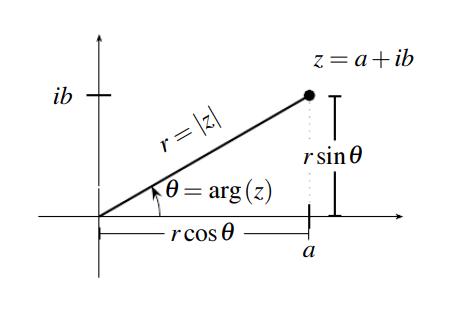
\includegraphics{../!assets/MATH1021-003-fig1.png}
    \caption{Polar form of complex numbers}
\end{figure}

\end{document}